\documentclass[11pt,a4paper]{article}
\usepackage[margin=21mm,headheight=16pt]{geometry}
\usepackage{fontspec}\setmainfont{Noto Serif}\setsansfont{Noto Sans}\setmonofont{Noto Sans Mono}
\usepackage{polyglossia}\setdefaultlanguage{turkish}
\usepackage{amsmath,amssymb,mathtools,graphicx,xcolor,booktabs,tabularx,array,enumitem}
\usepackage[most]{tcolorbox}\usepackage{fancyhdr,titlesec,needspace}
\usepackage[unicode,hidelinks,breaklinks]{hyperref}\usepackage{bookmark}
\definecolor{ink}{HTML}{18233A}\definecolor{accent}{HTML}{545AC4}\definecolor{green}{HTML}{087E66}\definecolor{paper}{HTML}{F3F5FA}
\color{ink}\setlength{\parindent}{0pt}\setlength{\parskip}{7pt}\linespread{1.10}
\setlength{\emergencystretch}{3em}\allowdisplaybreaks
\setlist{topsep=4pt,itemsep=4pt,leftmargin=*}
\pagestyle{fancy}\fancyhf{}\fancyhead[L]{\sffamily\small MÜHENDİSLİK MATEMATİĞİ}\fancyhead[R]{\sffamily\small Ders çalışma notları}\fancyfoot[L]{\sffamily\scriptsize Fotoğraflar + müfredat | 8 Kasım 2026}\fancyfoot[R]{\sffamily\thepage}
\titleformat{\section}{\Large\sffamily\bfseries\color{accent}}{\thesection}{.6em}{}
\titleformat{\subsection}{\large\sffamily\bfseries}{\thesubsection}{.6em}{}
\tcbset{enhanced,breakable,boxrule=.4pt,arc=2mm,left=3mm,right=3mm,top=2mm,bottom=2mm,before skip=8pt,after skip=8pt,fonttitle=\sffamily\bfseries,colback=paper,colframe=accent,coltitle=white}
\newcommand{\notebox}[2]{\begin{tcolorbox}[title={#1},colframe=accent!70!black]#2\end{tcolorbox}}
\hypersetup{pdfauthor={Mühendislik Matematiği Çalışma Atölyesi},pdfsubject={Ders fotoğrafları ve altı başlıklı müfredata göre özgün Türkçe çalışma notları}}
\begin{document}

\hypersetup{pdftitle={Çok değişkenli fonksiyonlar, limit ve süreklilik}}
{\sffamily\small\color{accent} ÇALIŞMA ATÖLYESİ / KONU 04\par}
\vspace{8mm}
{\Huge\sffamily\bfseries\raggedright\hyphenpenalty=10000 Çok değişkenli fonksiyonlar, limit ve süreklilik\par}
\vspace{3mm}
{\large Tanım bölgeleri, seviye eğrileri, komşuluklar, yol testi ve sıkıştırma ile limit.\par}
\vspace{4mm}\hrule\vspace{4mm}\subsection*{Bu bölümün hedefleri}\begin{itemize}
\item Tanım kümesini eşitsizliklerle ve bir çizimle ifade etmek.
\item Limitin yokluğunu iki yolla göstermek; varlığını tüm yollar için kanıtlamak.
\item Parçalı tanımlı bir fonksiyonun sürekliliğini incelemek.\end{itemize}
{\small\tableofcontents}\clearpage
\section{Birden fazla girdiye sahip fonksiyon}
\(f:D\subseteq\mathbb R^2\to\mathbb R\) fonksiyonu her \((x,y)\) noktasına bir sayı atar. Grafik \(z=f(x,y)\) uzayda bir yüzeydir; tanım kümesi ise \(xy\) düzlemindedir. Örneğin \(A(a,h)=ah/2\) üçgen alanı iki değişkenlidir; \(V(x,y,h)=xyh\) kutu hacmi üç değişkenlidir. Üç değişkenli skaler fonksiyonun grafiği dört boyutlu olur; seviye yüzeyleriyle görselleştirilir.

Tanım kümesi \(D\), fonksiyonun gerçek değer almasını sağlayan bütün girdilerdir. Görüntü kümesi \(f(D)\) ise gerçekten ulaşılabilen çıktılardır. Bir ifadede birden fazla kısıt varsa hepsi aynı anda sağlanmalıdır.

\begin{enumerate}
\item Karekök içi en az 0 olmalı.
\item Logaritma içi kesinlikle pozitif olmalı.
\item Payda sıfır olamaz.
\item \(\arcsin u\) ve \(\arccos u\) için \(-1\le u\le1\).
\end{enumerate}
\Needspace{14\baselineskip}\section{Dersteki tanım bölgesi örnekleri}
\Needspace{10\baselineskip}\begin{tcolorbox}[title={Örnek 4.1 | Disk ve eğik şerit},colframe=accent]\(f(x,y)=\sqrt{64-x^2-y^2}\) ve \(g(x,y)=\arccos(x-y)\) için tanım ve görüntü kümelerini bulunuz.
\par\vspace{1mm}{\scriptsize\sffamily Ders fotoğrafından | \nolinkurl{IMG-20261015-WA0041.jpg}}\end{tcolorbox}
\begin{tcolorbox}[title={Adım adım çözüm},colback=green!3!white,colframe=green]\begin{enumerate}
\item İlkinde \(x^2+y^2\le64\): merkezi orijin, yarıçapı 8 olan kapalı disk. Çıktılar \([0,8]\); grafik üst yarım küredir.
\item İkincide \(-1\le x-y\le1\), yani \(x-1\le y\le x+1\). Sınır doğruları dahil bir şerit. Görüntü \([0,\pi]\).
\end{enumerate}\end{tcolorbox}
\Needspace{10\baselineskip}\begin{tcolorbox}[title={Örnek 4.2 | Kök ve logaritmayı birlikte ele almak},colframe=accent]\(f(x,y)=\sqrt{xy}+\log(1-x^2-y^2)\) fonksiyonunun tanım bölgesini bulunuz.
\par\vspace{1mm}{\scriptsize\sffamily Ders fotoğrafından | \nolinkurl{IMG-20261015-WA0042.jpg}}\end{tcolorbox}
\begin{tcolorbox}[title={Adım adım çözüm},colback=green!3!white,colframe=green]\begin{enumerate}
\item \(xy\ge0\) ve \(x^2+y^2<1\) birlikte gerekli.
\item Bölge açık birim diskin birinci ve üçüncü bölgelerde kalan parçaları ile disk içindeki eksen parçalarıdır. Eksenler dahildir; çember dahil değildir.
\end{enumerate}\end{tcolorbox}
\Needspace{10\baselineskip}\begin{tcolorbox}[title={Örnek 4.3 | İşaret ayırımı gerektiren kök},colframe=accent]\(f(x,y)=\sqrt{xy-x^4}+xy\) ve \(g(x,y)=\sqrt{x^2-y}+x^2+y^2+1\) tanım bölgelerini bulunuz.
\par\vspace{1mm}{\scriptsize\sffamily Ders fotoğrafından | \nolinkurl{IMG-20261022-WA0053.jpg}}\end{tcolorbox}
\begin{tcolorbox}[title={Adım adım çözüm},colback=green!3!white,colframe=green]\begin{enumerate}
\item İlkinde \(x(y-x^3)\ge0\). \(x>0\) iken \(y\ge x^3\), \(x<0\) iken \(y\le x^3\); \(x=0\) iken her y geçerlidir. Sonuç \(\{x>0,y\ge x^3\}\cup\{x<0,y\le x^3\}\cup\{x=0\}\).
\item İkincide \(y\le x^2\). Parabol ve altı dahildir. İlk soruda x ile bölmeden önce x işareti ayrılmazsa bölgenin yarısı kaybolur.
\end{enumerate}\end{tcolorbox}
\Needspace{10\baselineskip}\begin{tcolorbox}[title={Örnek 4.4 | Her yerde tanımlı logaritma},colframe=accent]\(\ln(x^2+y^2+4)\) için tanım kümesi nedir?
\par\vspace{1mm}{\scriptsize\sffamily Ders fotoğrafından | \nolinkurl{IMG-20261022-WA0053.jpg}}\end{tcolorbox}
\begin{tcolorbox}[title={Adım adım çözüm},colback=green!3!white,colframe=green]\begin{enumerate}
\item \(x^2+y^2+4\ge4>0\) her noktada doğrudur. Dolayısıyla tanım kümesi \(\mathbb R^2\).
\item Logaritma artan olduğundan görüntü kümesi \([\ln4,\infty)\).
\end{enumerate}\end{tcolorbox}
\section{Seviye eğrileri ve seviye yüzeyleri}
\(f(x,y)=c\) denklemi aynı fonksiyon değerine sahip girdileri birleştirir. Haritadaki eş yükseklik eğrileri buna örnektir. Seviye eğrisi \(xy\) düzlemindedir; yüzey üzerinde \(z=c\) kesitinin düzleme izdüşümü olarak düşünülebilir. \(F(x,y,z)=c\) ise üç boyutlu uzayda bir seviye yüzeyidir.

\Needspace{10\baselineskip}\begin{tcolorbox}[title={Örnek 4.5 | Paraboloidin seviye eğrileri},colframe=accent]\(f(x,y)=x^2+y^2\) için \(c=0,1,4\) seviyelerini bulunuz.
\par\vspace{1mm}{\scriptsize\sffamily Ders fotoğrafından | \nolinkurl{IMG-20261015-WA0042.jpg}}\end{tcolorbox}
\begin{tcolorbox}[title={Adım adım çözüm},colback=green!3!white,colframe=green]\begin{enumerate}
\item \(c=0\) için yalnızca orijin, \(c=1\) için yarıçapı 1 çember, \(c=4\) için yarıçapı 2 çember vardır.
\item \(c<0\) için seviye kümesi boştur. Yüzey \(z=x^2+y^2\) yukarı açılan paraboloiddir.
\end{enumerate}\end{tcolorbox}
\begin{center}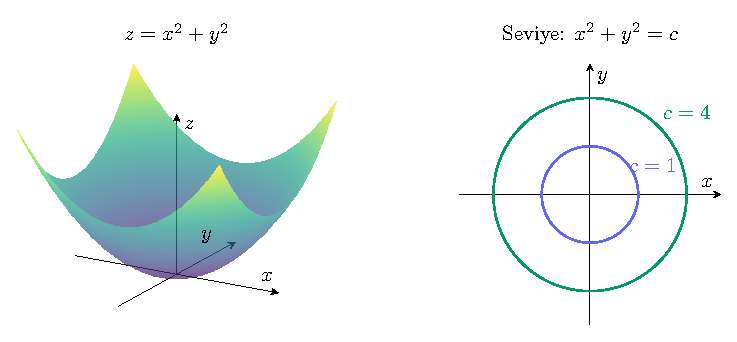
\includegraphics[width=.94\linewidth,height=65mm,keepaspectratio]{../assets/figures/levels.pdf}\par{\small\sffamily Aynı yüzey hem üç boyutlu grafik hem iki boyutlu seviye eğrileriyle okunabilir.}\end{center}
\section{Komşuluk ve limitin tam anlamı}
\((a,b)\) merkezli, yarıçapı \(\delta\) olan açık disk bir komşuluktur. Limit tanımında merkez nokta dışarıda bırakılır. Yaklaşım yalnızca tanım kümesindeki noktalardan yapılır. \((a,b)\), bu kümenin bir yığılma noktası olmalıdır.


{\small\[
\lim_{(x,y)\to(a,b)}f(x,y)=L\ \Longleftrightarrow\ \forall\varepsilon>0\ \exists\delta>0:\ 0<\sqrt{(x-a)^2+(y-b)^2}<\delta\ \Longrightarrow\ |f(x,y)-L|<\varepsilon.
\]}
Burada tek bir \(\delta\), izin verilen bütün yaklaşım yönlerini aynı anda kontrol etmelidir. Bu nedenle iki eksen üzerinde aynı sonucu bulmak limitin varlığını kanıtlamaz. Buna karşılık iki farklı yol üzerinde farklı sonuç bulmak limitin yokluğunu kanıtlamaya yeter.

\notebox{Doğru testi tek başına yeterli değildir}{Bütün \(y=mx\) doğruları aynı sonucu verse bile bir parabolda başka sonuç çıkabilir. Varlık için süreklilik, cebirsel dönüşüm veya tüm yönler için geçerli bir üst sınır kullan.}
\section{Süreklilik ve doğrudan yerine koyma}
Bir fonksiyon noktada tanımlıysa ve limiti değerine eşitse o noktada süreklidir. Polinomlar her yerde, rasyonel fonksiyonlar paydaları sıfır olmayan yerde süreklidir. Sürekli fonksiyonların uygun bileşkeleri de süreklidir. Bu kurallar uygunsa en kısa çözüm doğrudan yerine koymaktır.

\Needspace{10\baselineskip}\begin{tcolorbox}[title={Örnek 4.6 | Polinom limiti},colframe=accent]\(P(x,y)=5x^2y^2+4xy^3-8xy^2+3\) için \((x,y)\to(1,2)\) limitini bulunuz.
\par\vspace{1mm}{\scriptsize\sffamily Ders fotoğrafından | \nolinkurl{IMG-20261022-WA0053.jpg}}\end{tcolorbox}
\begin{tcolorbox}[title={Adım adım çözüm},colback=green!3!white,colframe=green]\begin{enumerate}
\item Polinom her yerde süreklidir; limit \(P(1,2)\).
\item \(5\cdot1\cdot4+4\cdot1\cdot8-8\cdot1\cdot4+3=20+32-32+3=23\).
\end{enumerate}\end{tcolorbox}
\Needspace{10\baselineskip}\begin{tcolorbox}[title={Örnek 4.7 | Dersin kısa limitleri},colframe=accent]\(\lim_{(x,y)\to(0,0)}(2x^2+y^2+1)/(x^2+y^2+3)\), \(\lim_{(x,y)\to(0,\ln2)}e^{x-y}\), \(\lim_{(x,y)\to(1,0)}x\sin y/(x^2+1)\) nedir?
\par\vspace{1mm}{\scriptsize\sffamily Ders fotoğrafından | \nolinkurl{IMG-20261022-WA0053.jpg}}\end{tcolorbox}
\begin{tcolorbox}[title={Adım adım çözüm},colback=green!3!white,colframe=green]\begin{enumerate}
\item İlk payda 3 olur; limit \(1/3\).
\item İkinci ifade süreklidir: \(e^{-\ln2}=1/2\).
\item Üçüncü payda 2 ve sinüs sıfır olur; limit 0.
\end{enumerate}\end{tcolorbox}
\Needspace{14\baselineskip}\section{Belirsizlikte cebir ve standart limitler}
\Needspace{10\baselineskip}\begin{tcolorbox}[title={Örnek 4.8 | Eşlenikle sadeleştirme},colframe=accent]\(\lim_{(x,y)\to(0,0)}[2-\sqrt{xy+4}]/(xy)\) hesaplayınız.
\par\vspace{1mm}{\scriptsize\sffamily Ders fotoğrafından | \nolinkurl{IMG-20261022-WA0053.jpg}}\end{tcolorbox}
\begin{tcolorbox}[title={Adım adım çözüm},colback=green!3!white,colframe=green]\begin{enumerate}
\item İfade kendi tanım kümesinde \(xy\ne0\) koşuluyla incelenir. Eşlenikle çarpınca pay \(4-(xy+4)=-xy\).
\item Yakında \(-1/[2+\sqrt{xy+4}]\) ile aynı olur. Bu sürekli ifadenin limiti \(-1/4\). Fonksiyonun eksenlerde tanımsız olması limit almayı engellemez.
\end{enumerate}\end{tcolorbox}
\Needspace{10\baselineskip}\begin{tcolorbox}[title={Örnek 4.9 | Sinüs içeren limitler},colframe=accent]\(\lim_{(x,y)\to(0,0)}\sin(xy)/x\) ve \(\lim_{(x,y)\to(0,0)}e^y\sin x/x\) hesaplayınız.
\par\vspace{1mm}{\scriptsize\sffamily Ders fotoğrafından | \nolinkurl{IMG-20261022-WA0056.jpg}}\end{tcolorbox}
\begin{tcolorbox}[title={Adım adım çözüm},colback=green!3!white,colframe=green]\begin{enumerate}
\item İlk ifade, uygun noktalarda \(y[\sin(xy)/(xy)]\) olur. Standart \(\sin u/u\to1\) limiti ve \(y\to0\) ile sonuç 0. Doğrudan \(|\sin(xy)/x|\le|y|\) sınırı da aynı sonucu verir.
\item İkincide \(e^y\to1\) ve \(\sin x/x\to1\); sonuç 1. Her iki limitte yaklaşım fonksiyonun tanımlı olduğu noktalar üzerindendir.
\end{enumerate}\end{tcolorbox}
\Needspace{14\baselineskip}\section{İki farklı yolla limitin yokluğu}
\Needspace{10\baselineskip}\begin{tcolorbox}[title={Örnek 4.10 | Doğruya bağlı sonuç},colframe=accent]\(f(x,y)=2xy/(x^2+y^2)\) için orijindeki limiti inceleyiniz.
\par\vspace{1mm}{\scriptsize\sffamily Ders fotoğrafından | \nolinkurl{IMG-20261022-WA0058.jpg}}\end{tcolorbox}
\begin{tcolorbox}[title={Adım adım çözüm},colback=green!3!white,colframe=green]\begin{enumerate}
\item \(y=0\) yolunda değer 0; \(y=x\) yolunda, \(x\ne0\) için değer 1.
\item İki yol aynı noktaya gider fakat sonuçlar farklıdır. Dolayısıyla limit yoktur. Genel \(y=mx\) yolunda \(2m/(1+m^2)\) çıkar.
\end{enumerate}\end{tcolorbox}
\Needspace{10\baselineskip}\begin{tcolorbox}[title={Örnek 4.11 | Parabol yoluyla limitin yokluğu},colframe=accent]\(f(x,y)=(x^4-y^2)/(x^4+y^2)\) için orijindeki limiti inceleyiniz.
\par\vspace{1mm}{\scriptsize\sffamily Ders fotoğrafından | \nolinkurl{IMG-20261022-WA0056.jpg}}\end{tcolorbox}
\begin{tcolorbox}[title={Adım adım çözüm},colback=green!3!white,colframe=green]\begin{enumerate}
\item \(y=0\) boyunca değer 1; \(y=x^2\) boyunca değer 0. İki sonuç farklı, limit yok.
\item Genel \(y=ax^2\) yolunda \((1-a^2)/(1+a^2)\) çıkar. Bu örnek, paydadaki dereceleri eşleştirerek uygun yol seçmeyi öğretir.
\end{enumerate}\end{tcolorbox}
\Needspace{10\baselineskip}\begin{tcolorbox}[title={Örnek 4.12 | İki başka karşı örnek},colframe=accent]\((x-y)/(x+y)\), \(x/\sqrt{x^2+y^2}\) ve \((x^2+y^2)/y^2\) orijinde limite sahip midir?
\par\vspace{1mm}{\scriptsize\sffamily Ders fotoğrafından | \nolinkurl{IMG-20261022-WA0054.jpg}}\end{tcolorbox}
\begin{tcolorbox}[title={Adım adım çözüm},colback=green!3!white,colframe=green]\begin{enumerate}
\item İlkinde \(y=0\) yolu 1, \(x=0\) yolu -1 verir. İkinci ifadede pozitif x ekseni 1, negatif x ekseni -1 verir. İkisinin de limiti yoktur.
\item Üçüncüde y sıfır olamaz; \(y=x\) yolunda 2, \(y=2x\) yolunda \(5/4\) çıkar. Bu limit de yoktur. Tanımsız yolları test yolu olarak seçme.
\end{enumerate}\end{tcolorbox}
\section{Kutupsal koordinatlar ve sıkıştırma}
Orijine yaklaşırken \(x=r\cos\theta,y=r\sin\theta\), \(r\to0^+\) dönüşümü yararlıdır. Ancak sabit bir açı seçmek yalnızca bir ışını test eder. Limitin varlığını göstermek için \(\theta\) ne olursa olsun sıfıra giden bir sınır bulunmalıdır. Örneğin \(|r\cos\theta\sin^2\theta|\le r\) eşitsizliği böyle bir sınırdır.

\Needspace{10\baselineskip}\begin{tcolorbox}[title={Örnek 4.13 | Dersteki parçalı fonksiyonun sürekliliği},colframe=accent]\(f(x,y)=\sin(xy^2)/(x^2+y^2)\) orijin dışında, \(f(0,0)=0\) olsun. Her yerde sürekli olduğunu gösteriniz.
\par\vspace{1mm}{\scriptsize\sffamily Ders fotoğrafından | \nolinkurl{IMG-20261022-WA0054.jpg}}\end{tcolorbox}
\begin{tcolorbox}[title={Adım adım çözüm},colback=green!3!white,colframe=green]\begin{enumerate}
\item Orijin dışında payda sıfır değildir, dolayısıyla süreklidir. Orijinde \(|\sin u|\le|u|\) kullanılır.
\item \(|f(x,y)|\le |x|y^2/(x^2+y^2)\le|x|\le\sqrt{x^2+y^2}\to0\). Böylece limit 0 olur ve atanmış değere eşittir.
\item Kutupsal yazım da sınırı \(r|\cos\theta|\sin^2\theta\le r\) yapar. Bu tüm açılar için geçerli olduğu için kanıttır.
\end{enumerate}\end{tcolorbox}
\begin{center}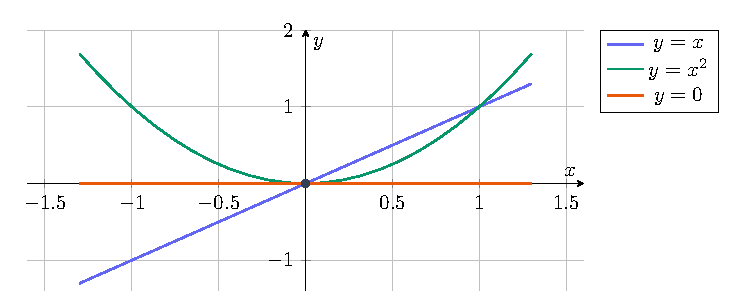
\includegraphics[width=.94\linewidth,height=65mm,keepaspectratio]{../assets/figures/paths.pdf}\par{\small\sffamily Aynı noktaya farklı yollarla yaklaşılır. Limitin varlığı bütün bu yolları aynı anda kapsar.}\end{center}
\section{Limit için uygulanabilir karar sırası}
\begin{enumerate}
\item Önce tanım kümesini ve noktanın yığılma noktası olup olmadığını kontrol et.
\item Süreklilik uygunsa yerine koy. Belirsizlik varsa eşlenik veya çarpanlara ayırma dene.
\item Yokluk şüphesinde iki uygun yol seç; farklı sonuç bulunca kanıt tamamdır.
\item Varlık şüphesinde sıkıştırma veya açıdan bağımsız bir kutupsal üst sınır kur.
\item Parçalı tanımda bulunan limiti atanmış nokta değeriyle karşılaştır.
\end{enumerate}
\Needspace{10\baselineskip}\begin{tcolorbox}[title={Örnek 4.14 | Bütün doğruların aynı sonucu vermesi yetmez},colframe=accent]\(f(x,y)=x^2y/(x^4+y^2)\) orijinde limite sahip midir?
\par\vspace{1mm}{\scriptsize\sffamily Pekiştirme}\end{tcolorbox}
\begin{tcolorbox}[title={Adım adım çözüm},colback=green!3!white,colframe=green]\begin{enumerate}
\item \(y=mx\) ve sabit \(m\ne0\) için \(f=mx/(x^2+m^2)\to0\). \(m=0\) ve dikey eksen de 0 verir.
\item Fakat \(y=x^2\) boyunca \(f=1/2\). Bu nedenle limit yoktur. Bütün doğruların kontrol edilmesi bile genel limit için yeterli değildir.
\end{enumerate}\end{tcolorbox}

\clearpage
\section*{Kaynaklar ve kapsam}
\addcontentsline{toc}{section}{Kaynaklar ve kapsam}
Bu metin 156 ders/defter fotoğrafı ve altı başlıklı müfredata göre özgün olarak yazıldı. Fotoğraflar dersin sıra ve örneklerini belirler. Ek sorular pekiştirme olarak etiketlidir; çıkmış sınav sorusu iddiası yoktur. Soluk semboller tahminle aktarılmadı. Gradyan ve yönlü türev, müfredat gereği tamamlanan anlatımdır. Fotoğraf bazında inceleme dizini web sitesinde ve analysis/FOTOGRAF\_INCELEMESI.md dosyasında bulunur.
\textbf{Birincil ders malzemesi}. Kullanıcının sağladığı 156 JPG ders/defter fotoğrafı ve mufredat.png. Dosya tarihleri ders tarihi olarak varsayılmadı. Konu-fotoğraf eşleştirmesi fotoğraf dizinindedir.\par
\textbf{Erwin Kreyszig · Advanced Engineering Mathematics}. Dersin belirtilen kitabı. Wiley 10. baskı bölüm diziniyle vektör diferansiyel hesabı başlığı eşleştirildi; tam kitap dosyası sağlanmadı. Kitaptan birebir metin veya soru aktarımı yapılmadı.
{\footnotesize\url{https://bcs.wiley.com/he-bcs/Books?action=contents&bcsId=6140&itemId=0470458364}}\par
\textbf{KOCW · Kreyszig temelli Bölüm 9 ders notları}. Sungkyunkwan / Kim Munhyeon, vektörler ve vektör fonksiyonları. Açık üniversite notu kavram ve formül kontrolünde kullanıldı. Buradaki Türkçe açıklamalar ve çözümler özgün olarak yazıldı.
{\footnotesize\url{https://contents.kocw.net/KOCW/document/2015/sungkyunkwan/kimmunhyeon3/8.pdf}}\par
\textbf{Zill ve Wright · Calculus / Matematik}. Kullanıcının verdiği bibliyografya: İ. N. Cangül çevirisi, Nobel, 2013. Tam metne erişilmedi; baskıya özgü sayfa ve soru numarası atfedilmedi.\par
\textbf{Mustafa Balcı · Genel Matematik II}. Kullanıcının verdiği bibliyografya: Sürat, 2013. Tam metin sağlanmadı; bu kitaptan doğrulanmış alıntı veya sayfa atfı yapılmadı.\par
\textbf{MIT OCW · 18.02 ders notları}. Denis Auroux, 2007. Ders düzeni ve kavram denetimi için açık ders dizini. Müfredat dışındaki çok katlı integraller ve integral teoremleri bu çalışmaya eklenmedi.
{\footnotesize\url{https://ocw.mit.edu/courses/18-02-multivariable-calculus-fall-2007/pages/lecture-notes/}}\par
\textbf{MIT · Teğet düzlem ve gradyan}. Gradyanın teğet düzlem ve yönlü türevle ilişkisi için açık teknik kontrol kaynağı. Konuya eklenen örnekler özgün pekiştirme sorularıdır.
{\footnotesize\url{https://www.ocw.mit.edu/ans7870/18/18.013a/textbook/HTML/chapter06/section05.html}}\par
\end{document}
